\section{Evidence on $S$}
\label{sec:S-evidence}

\subsection{Recognition curves on controlled images}
\label{sec:S-curves}

\begin{figure*}[t]
\centering
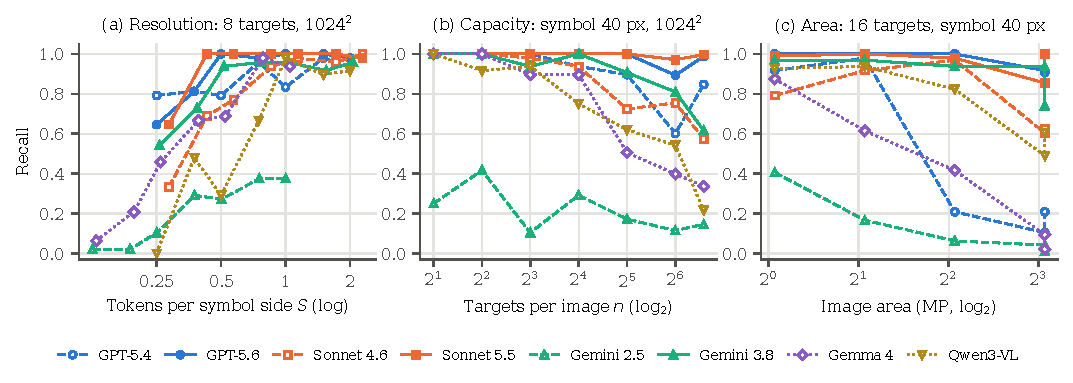
\includegraphics[width=\textwidth]{figures_x/fig_syn.pdf}
\caption{Controlled images, eight models. (a) Recall against $S$ (8 targets and 8 distractors on $1024^2$). (b) Recall against the number of targets per call at fixed $S$ (1.25 to 1.43 for resolution-scaled models; symbol 40 px on $1024^2$). (c) Recall against image area with 16 targets of fixed pixel size. Dashed and hollow: older generation; solid and filled: newer generation. Six images per point; mean matched recall per image; no intervals shown. Panels (a) and (b) are \cref{fig:curves}.}
\label{fig:syn}
\end{figure*}

\begin{table*}[t]
\centering
\footnotesize
\setlength{\tabcolsep}{4pt}
\begin{adjustbox}{max width=\linewidth}\begin{tabular}{lcccccc}
\toprule
 & \multicolumn{2}{c}{Recognition} & \multicolumn{3}{c}{Target count (fixed $S$)} & Area \\
\cmidrule(lr){2-3}\cmidrule(lr){4-6}\cmidrule(lr){7-7}
Model & $S_{50}$ & R($S{<}0.5$) & $S$ & R, $n{=}2 \to 96$ & slope & R, 1 $\to$ 8.4 megapixels ($S$) \\
\midrule
\inputrows{generated_x/tab_syn.tex}
\bottomrule
\end{tabular}\end{adjustbox}
\caption{Controlled images. $S_{50}$: the $S$ at which recall reaches one half (logistic fit of per-image recall on $\log S$; $<$0.25: below 0.25, extrapolated below the smallest $S$ tested). R($S{<}0.5$): mean recall over images with $S < 0.5$. Target count: $1024^2$ canvas, symbol 40 px, $n$ targets and $n$ distractors; slope of recall per doubling of $n$. Area: 16 targets at 40 px on canvases from $1024^2$ to $4096 \times 2048$, with $S$ on the largest canvas in brackets. Upper block: older generation; lower block: newer generation.}
\label{tab:syn}
\end{table*}

Recall rises with $S$ for every model, gradually rather than at a sharp threshold, and the level at which it rises differs by model (\cref{fig:syn}a, \cref{tab:syn}). Gemini 2.5 needs about one token per target side ($S_{50} = \XSfiftygeminiTwoFive$, interval \XSfiftyCIgeminiTwoFive). Gemma 4, Claude Sonnet 4.6 and Qwen3-VL reach one half at \XSfiftygemmaFour{} \XSfiftyCIgemmaFour, \XSfiftysonnetFourSix{} \XSfiftyCIsonnetFourSix{} and \XSfiftyqwenThreevl{} \XSfiftyCIqwenThreevl. GPT-5.4, GPT-5.6, Gemini 3.8 and Claude Sonnet 5.5 reach it near or below the smallest $S$ we tested for them (0.13 to 0.29), so their values (\XSfiftygptFiveFour, \XSfiftygptFiveSix, \XSfiftygemThreeEight, \XSfiftysonnetFiveFive) rest on extrapolation. Clutter, 0 to 640 grey segments per megapixel, changes recall little: the slope per doubling of the segment density has an interval containing zero for every model (for example GPT-5.6 \XclutSlopegptFiveSix{} \XclutSlopeCIgptFiveSix). The difference between models is not geometric. At Gemini 3.8's low budget its token grid is the same as Gemini 2.5's default grid, yet its recall on the same images is higher by \XtOneHThree{} \XtOneHThreeCI.

\subsection{The same pixels at three budgets}
\label{sec:budget}

Gemini 3.8 lets the caller set the token budget per image while the pixels stay fixed: about 257, 1{,}090 or 2{,}210 tokens. On the resolution sweep, recall of 8 px targets rises from \CbudEightLo{} to \CbudEightDef{} to \CbudEightUh{} across the three budgets. A logistic curve in $\log S$ captures most of this; adding a separate offset per budget fits better (difference in Akaike information criterion, $\Delta\mathrm{AIC} = \XtOneDAIC$), so the budget also acts beyond $S$. On floor-plan mosaics, raising the budget from low to default changes F1 by \XfTOnesheetssmallDL{} \XfTOnesheetssmallDLCI{} on the \XfTOnesheetssmallN{} items whose low-budget $S$ is below 1.5 and by \XfTOnesheetslargeDL{} \XfTOnesheetslargeDLCI{} on the other \XfTOnesheetslargeN; on floor-plan blocks the two gains are \XfTOnebenchsmallDL{} \XfTOnebenchsmallDLCI{} and \XfTOnebenchlargeDL{} \XfTOnebenchlargeDLCI. Raising it further, from default to ultra-high, changes F1 by at most \XfTOnesheetslargeUD{} in any of these groups, none significantly: the gain is concentrated where $S$ is low.

\subsection{Dose response on drawings and floor plans}
\label{sec:dose}

\begin{figure}[t]
\centering
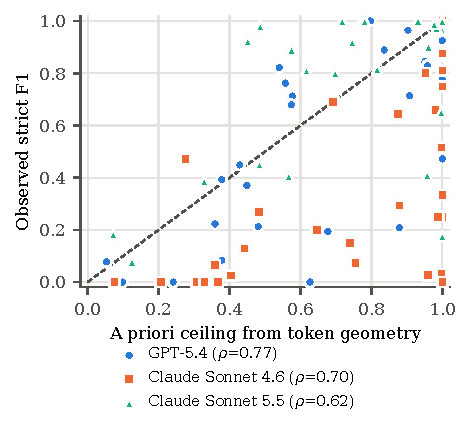
\includegraphics[width=0.92\columnwidth]{figures_x/fig_dose.pdf}
\caption{Whole-image F1 per LegendSpot test drawing against a ceiling computed from the token geometry before any call (34 drawings; dashed line: observed equals ceiling), for three models. F1 under one-to-one matching (axis: strict F1); Spearman $\rho$ for every model in the text.}
\label{fig:dose}
\end{figure}

For each LegendSpot test drawing we computed a ceiling from the geometry alone, before any call, by simulating the token-quantized observer of \cref{prop:loc}: instances that share a token cell merge into one report at the cell centre. Whole-image F1 follows it (\cref{fig:dose}; Spearman $\rho = \RhogptFiveFour$ \RhogptFiveFourCI{} for GPT-5.4, \RhosonnetFourSix{} \RhosonnetFourSixCI{} for Claude Sonnet 4.6, \RhogemmaFour{} \RhogemmaFourCI{} for Gemma 4, \RhogeminiTwoFive{} \RhogeminiTwoFiveCI{} for Gemini 2.5, \RhoqwenThreevl{} \RhoqwenThreevlCI{} for Qwen3-VL, \RhogptFiveFive{} for GPT-5.5, \RhogptFiveSix{} for GPT-5.6, \RhosonnetFiveFive{} for Claude Sonnet 5.5, \RhoopusFiveFive{} for Claude Opus 5.5, and \RhogemThreeEight{} \RhogemThreeEightCI{} for Gemini 3.8, the only interval including zero). Tiles help where the ceiling is low (\GainLowgptFiveFour{} F1 for GPT-5.4) and not where it is high (\GainHighgptFiveFour{} \GainHighgptFiveFourCI). The ceiling is a function of $S$ and of how often instances share a token, and $\log S$ alone explains as much of the per-drawing variance ($R^2$ \XtTwoRSgptFiveFour{} against \XtTwoRCgptFiveFour{} for GPT-5.4, \XtTwoRSsonnetFourSix{} against \XtTwoRCsonnetFourSix{} for Claude Sonnet 4.6), so we treat $S$ as the operative variable and the ceiling as a reference line. On floor-plan mosaics, pooled over the three areas, per-item F1 again rises with $S$ for every model (Spearman \XfHEightgptFiveSix{} for GPT-5.6, \XfHEightsonnetFiveFive{} for Claude Sonnet 5.5, \XfHEightgemThreeEight{} for Gemini 3.8).

\subsection{Generations}
\label{sec:generations}

\begin{figure*}[t]
\centering
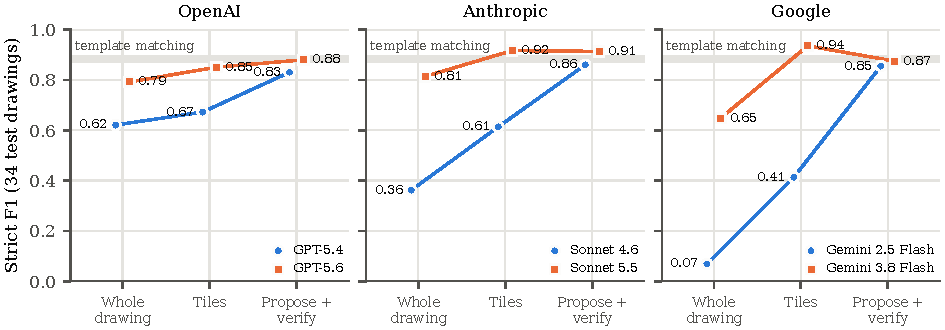
\includegraphics[width=0.95\textwidth]{figures_x/fig_generations.pdf}
\caption{Two generations per vendor under three configurations (F1, 34 LegendSpot test drawings; whole image read in each model's published convention). Propose and verify: template matching proposes candidates and the model accepts or rejects each one, shown as a crop at the reference's scale. Grey band: template matching with two threshold choices. F1 under one-to-one matching (axis: strict F1); point estimates.}
\label{fig:gen}
\end{figure*}

Larger budgets raise whole-image F1 where geometry says they should (\cref{fig:gen}): by \CgenclaudeATwosheets{} \CgenclaudeATwosheetsCI{} on full sheets from Claude Sonnet 4.6 to 5.5 (1{,}568 to 4{,}784 tokens; Sonnet 5.5 also thinks adaptively), and by \CgengeminiATwosheets{} \CgengeminiATwosheetsCI{} from Gemini 2.5 to 3.8 (258 to about 1{,}090 tokens). At unchanged geometry GPT-5.6 improves on GPT-5.4 by \CgengptFiveSixAOne{} \CgengptFiveSixAOneCI, while GPT-5.5 does not (\CgengptFiveFiveAOne{} \CgengptFiveFiveAOneCI): recognition also improves across generations, though not monotonically.

\subsection{Enlargement}
\label{sec:enlarge}

\cref{prop:geometry} predicts that a fixed-grid model gains from a smaller field of view but not from more pixels, while a resolution-scaled model can gain from enlargement as long as the pixels resolve the target. Choosing Gemini 2.5's and Gemma 4's field of view by \cref{prop:geometry}(c) instead of the 44 px recipe adds \CDMinusCgeminiTwoFive{} \CDMinusCgeminiTwoFiveCI{} and \CDMinusCgemmaFour{} \CDMinusCgemmaFourCI{} F1 on LegendSpot, and enlarging controlled images twofold leaves fixed-grid recall unchanged (Gemini 3.8 \XupDgemThreeEight{} \XupDCIgemThreeEight, Gemma 4 \XupDgemmaFour{} \XupDCIgemmaFour). For resolution-scaled models enlargement adds tokens but no Shannon information (\cref{prop:dpi}), so it helps only when the pixels resolve the target but the tokens do not, and whether it helps depends on the recognizer: at 8 px, twofold enlargement raised GPT-5.6's recall from \XupEightgptFiveSix{} and left Claude Sonnet 5.5's unchanged (\XupEightsonnetFiveFive). GPT-5.4's recall changed by \XtcViolD{} \XtcViolCI{} on the enlarged images, which its vendor shrinks again; this is one of the four violations (\cref{sec:violations}).

\subsection{The newest generation}
\label{sec:newest}

To compare the newest models we measured, for each, the $S$ at which it first reaches recall and precision of 0.9 ($S_{90}$), at the vendor's default reasoning setting (no reasoning parameter sent) and with an output cap of 16{,}384 tokens. Each controlled image holds 8 targets of one type and distractors of three other types, laid out in 12 base scenes; each scene is rendered at a grid of $S$ values by scaling the whole scene, without blank padding for the resolution-scaled models and centred on a fixed $1024^2$ canvas for the fixed-grid models. $S_{90}$ is the smallest tested $S$ at which the pooled recall and precision both reach 0.9 and stay at or above 0.9 at every larger tested $S$ (a single failure at the largest $S$ alone does not count); 90\% intervals resample the base scenes (2{,}000 draws). \Cref{tab:newest} gives the results; Qwen3-VL, run through a second provider, does not reach 0.9 at the largest $S$ tested (2.8). On the same 1{,}090-token grid, the $S$ that Gemini 4 needs is less than half of Gemini 3.8's.

\begin{table}[t]
\centering
\small
\setlength{\tabcolsep}{4pt}
\begin{adjustbox}{max width=\linewidth}\begin{tabular}{lcc}
\toprule
Model & $S_{90}$ & 90\% interval \\
\midrule
GPT-5.6 & 0.64 & [0.53, 0.79] \\
GPT-6.1 & 0.57 & [0.44, 0.60] \\
Claude Opus 5.5 & 0.63 & [0.51, 0.73] \\
Gemini 3.8 & \CgenSninetyGemThreeEight & [0.58, 1.63] \\
Gemini 4 & \CgenSninetyGemFour & [0.21, 0.38] \\
\bottomrule
\end{tabular}\end{adjustbox}
\caption{The $S$ at which recall and precision reach 0.9 on controlled images, at each vendor's default reasoning. The 90\% intervals resample the 12 base scenes (2{,}000 draws).}
\label{tab:newest}
\end{table}

\paragraph{Rendering.} The rendering pastes only template pixels darker than 200 after Lanczos downscaling, so the lightest strokes of a symbol are dropped at small scales; the load sweep of \cref{sec:thumb} keeps them as grey.
